\documentclass[11pt]{article} %tamño de letra, tipo de artículo
\usepackage{fontspec}
% Configuración de la fuente Times New Roman
\setmainfont{Times New Roman}
\usepackage{setspace}    % Permite ajustar el espaciado entre líneas (simple, 1.5, doble).
\onehalfspacing
\usepackage{graphicx}    % Facilita la inclusión y manipulación de imágenes en el documento.
%\usepackage{geometry}    
\usepackage{amsmath}     % Mejora el entorno matemático de LaTeX para expresiones complejas.
\usepackage{natbib}      % Gestiona citas y referencias bibliográficas con estilos variados.
\usepackage{array}       % Amplía las capacidades de formateo de tablas en el entorno array.
\usepackage{multirow}    % Permite crear celdas que abarquen varias filas en tablas.
\usepackage{siunitx}     % (Reemplaza a dcolumn) Alinea columnas numéricas y maneja unidades de manera avanzada.
\usepackage{textcomp}    % Proporciona símbolos adicionales como el símbolo del grado, número y el euro.
\usepackage[utf8]{inputenc}  % Configura la codificación del documento para usar UTF-8.
%\usepackage[T1]{fontenc}     % Configura la salida del documento con codificación T1, adecuada para caracteres en español.
\usepackage[spanish,es-tabla]{babel}  % Configura el documento para usar el idioma español, ajustando reglas tipográficas y de separación de sílabas. le dice adicionalmente que las tablas se llaman tablas, no cuadros.
\usepackage{csquotes}        % Proporciona comillas tipográficas adecuadas para el español.
\usepackage[top=1in,right=1in,left=1in,bottom=1in]{geometry} % Ajusta los márgenes y la disposición de la página. Este indica que el margen es de una pulgada a cada lado.
\usepackage{makecell} % Para el comando \makecell

\bibpunct{(}{)}{;}{a}{}{,}
\parindent 1.5em %\raggedright

\usepackage{hyperref}        % Convierte referencias cruzadas y URLs en hipervínculos dentro del PDF.

\hypersetup{
    unicode=true,            % Permitir caracteres no latinos en los marcadores.
    pdftoolbar=true,         % Mostrar la barra de herramientas de Acrobat.
    pdfmenubar=true,         % Mostrar el menú de Acrobat.
    pdffitwindow=false,      % Ajustar la ventana a la página al abrir.
    pdfstartview={FitH},     % Ajusta el ancho de la página a la ventana.
    pdftitle={},             % Título del documento.
    pdfauthor={},            % Autor del documento.
    pdfsubject={},           % Asunto del documento.
    pdfcreator={},           % Creador del documento.
    pdfproducer={},          % Productor del documento.
    pdfkeywords={},          % Lista de palabras clave.
    pdfnewwindow=true,       % Abrir enlaces en una nueva ventana.
    colorlinks=true,         % Enlaces en color (sin recuadro).
    linkcolor=blue,          % Color de los enlaces internos.
    citecolor=blue,          % Color de los enlaces a la bibliografía.
    filecolor=blue,          % Color de los enlaces a archivos.
    urlcolor=blue            % Color de los enlaces externos.
}
\title{SOCI 4186-00N \\ Tarea \textnumero 1 - Ejercicio de aprendizaje de programaci\'on de \LaTeX.}

\author{Pon tu nombre aquí}

\date{\today}

\begin{document}


\maketitle
\begin{center}
   A entregarse el lunes 29 de agosto de 2025. 
\end{center}

Esta es la tarea para ustedes: 
\begin{enumerate}
    \item Descargarán este documento en el GitHub de la clase, y lo subirán a la misma carpeta que abrieron cuando hicieron cuenta conmigo en Overleaf el lunes (probablemente llamada Proyecto).
    \item Cambiarán el nombre que sale arriba (al final del preámbulo, poco antes del \texttt{\textbackslash begin\{document\}}, donde dice \texttt{\textbackslash author\{Pon tu nombre aquí\}} y pondrán en su lugar su nombre(s) y apellidos. También sustituirán la N por la sección (1 o 2).
    \item Prestarán atención a la ortografía de la lengua española, asegurándose de colocar acentos, diéresis, o tildes donde deban ir. Para esto, tienen dos opciones 
    \begin{enumerate}
        \item si su teclado estuviera en español, usen los símbolos donde es menester,
        \item si su teclado no estuviera en español, está la opción indicada en clase de usar \texttt{\textbackslash} y el símbolo necesario (por ejemplo, \textbackslash'\ para acento (\'a), \textbackslash "\  para diéresis (\"u), \textbackslash \~\ para \~n)
        \item Alternativamente, si prefiriera escribir en inglés \underline{la tarea entera}, podrá hacerlo, ciñéndose estrictamente a una de las tres ortografías principales de ese idioma, es decir, inglés británico, inglés Oxford, o inglés estadounidense.
    \end{enumerate}
    \item Completarán como mejor sea posible la tarea, y podrán, si entienden necesario hacerlo, trabajar la tarea con compañeres de clase. Si así lo hicieren, pondrán antes de la sección 1 una oración indicándome con quién(es) trabajó la tarea. De lo contrario, dejarán la línea que está actualmente escrita.
    \item  Una vez terminen, apretarán el símbolo de descarga (a la derecha del botón de Compilar, con flecha descendiente), y descargarán el PDF para enviarlo a mi persona.
    \item Someterán la tarea mediante la aplicación de Teams en la semana.
\end{enumerate}


\textbf{Declaro que soy la única persona que trabajó en solucionar esta tarea.}

\section{Problemas matemáticos}

Para los siguientes problemas, resuelva mostrando los pasos intermedios. Aquí un ejemplo, usando el ambiente demarcado por begin y end de \texttt{align}.

\begin{align*}
    2x - 6 &=  8 \\
    2x &= 8+6 \\
    2x &= 14 \\
    x &= 14/2 \\
    x &= 7
\end{align*}

Note el uso del símbolo \textbf{et} o \textit{ampersand} \&= como parte de cómo a través de código, la ecuación se alinea en el ejemplo. Si tiene dudas, no dude contactarnos por correo o venir a nuestras horas de oficina.

\subsection{Problema 1} 

Resuelva la ecuación siguiente: $-2x + 10 = 2x - 10$ usando \texttt{align} para mostrar los pasos intermedios.


\subsection{Problema 2} 

Resuelva la desigualdad: $4(2x - 5) > 7x + 8 - x$ usando \texttt{align} para mostrar los pasos intermedios.

\section{Temas de interés}

\subsection{La tablita}
Llene la siguiente tabla con información requerida. El propósito es el aprendizaje del manejo de la tabla. Si desea alterar el formato de modo distinto al presente (alinear el texto de una columna al centro o a la derecha o izquierda), podrá hacerlo, por ejemplo alterando el código de la tabla o el editor visual. Para la tabla, note, que he añadido algo adicional, arriba un paquete (\texttt{makecell}) y en la tabla, que he llenado con mi información, también hay dos de las cuatro celdas usando ese comando (note que usa \texttt{\textbackslash \textbackslash} para separar el texto y expandir la altura de la celda, para no salirse del margen de página).


\begin{table}[h!]
    \centering
    \caption{Tabla con información pedida}
    \label{tab:mi_tablita}
    \begin{tabular}{cccc}
    \\
    \hline
       Nombre y Apellidos & \textnumero de estudiante & Concentración & Temas de interés\\
    \hline
    Rashid C.J. Marcano Rivera & 801-06-4104 & \makecell{Ciencias políticas, \\ Música} & \makecell{Desigualdad social, \\ Capitalismo comparado, \\ Economía política} \\
    \hline
    \end{tabular}

\end{table}

 \subsection{La imagen}

Inserte una imagen (al tamaño que usted mejor entienda en relación con el ancho de página) que represente el o los temas que más le interesen de los que mencionara en el cuadro o tabla \ref{tab:mi_tablita}. Recuerde que tendrá que subir la imagen o hacer referencia a un enlace de URL (una de las opciones disponibles en los botones de importar o insertar imagen de arriba). Debajo de la imagen, incluya un pie de foto (caption) explicando qué es.  

\begin{figure}[h!]
    \centering
    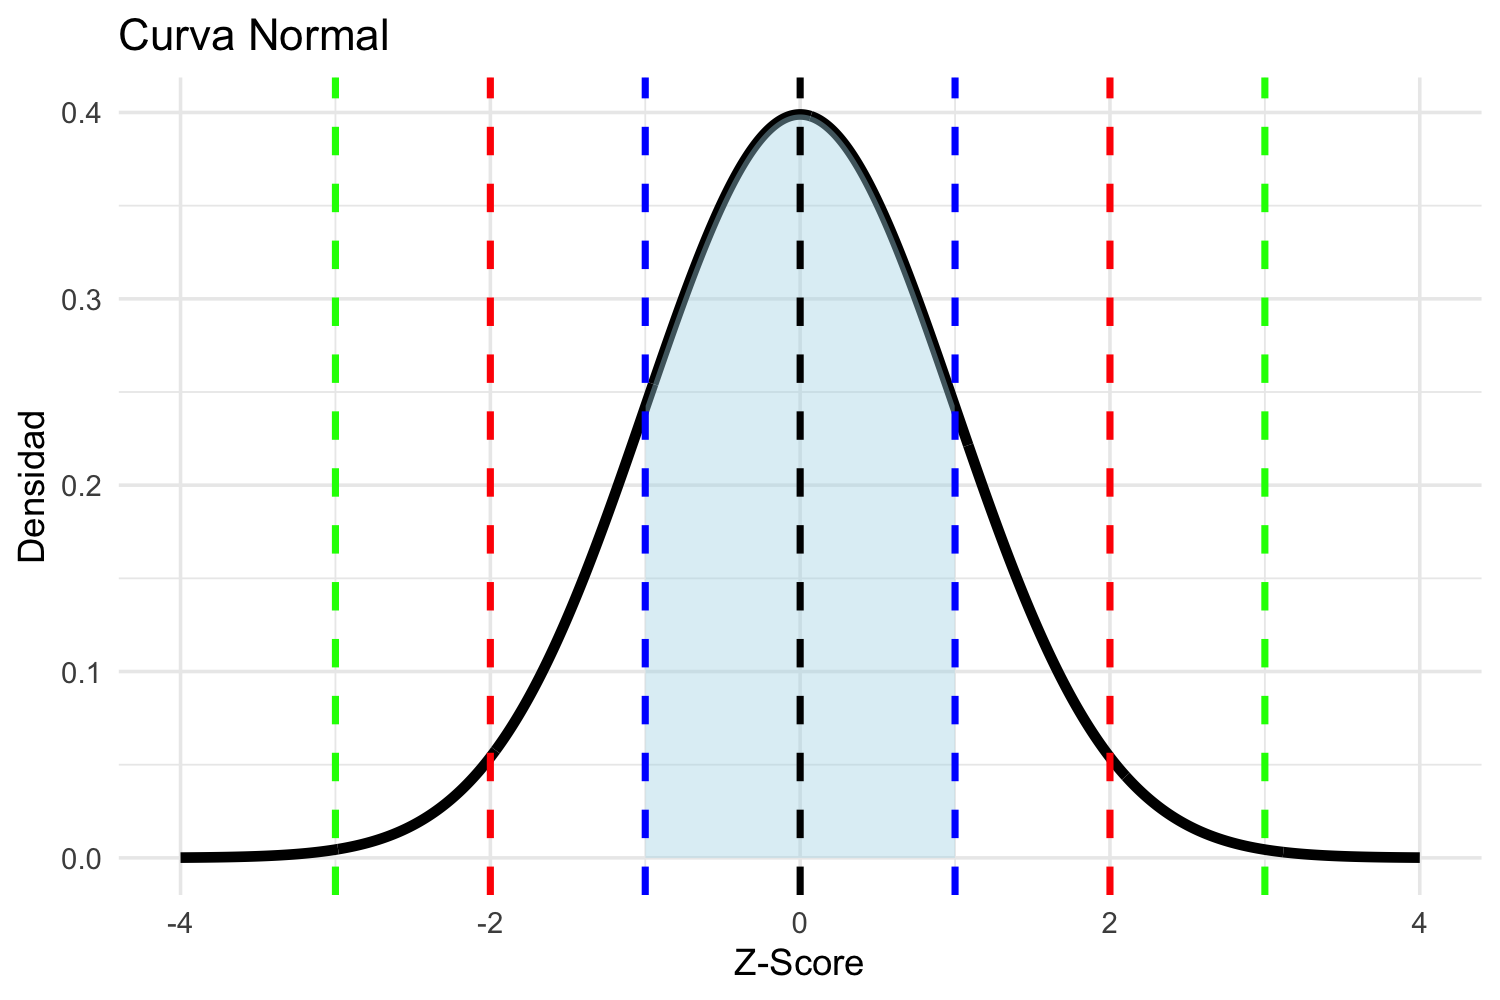
\includegraphics[width=0.9\linewidth]{Curva normal.png}
    \caption{Esta es la curva normal, para distribuci\'on $\sim N(\mu=0,\sigma^2=1$)}
    \label{fig:lafoto}
\end{figure}

\doublespacing
Finalmente, escriba un breve párrafo (unas 3 ó 4 oraciones) \underline{después de la imagen \ref{fig:lafoto}}, donde explique cuál de los temas le llama más la atención para explorar a fondo durante el curso y por qué. Use \textbf{negrita}, \textit{cursiva}, o \underline{subrayado} en algún momento durante ese párrafo para enfatizar algo que entienda sea importante que yo entienda.

\end{document}





